

% ------------------------------------------------------------------------------
% ------------------------------------------------------------------------------

%
% Optional reading
%

\begin{frame}[plain,c]
\begin{center}
{\Huge \bf Optional reading for Lecture \thislecture}
\end{center}
\end{frame}


%
%
%

\begin{frame}{Electric dipole field}

\begin{columns}
  \begin{column}{0.20\textwidth}
   \begin{center}
     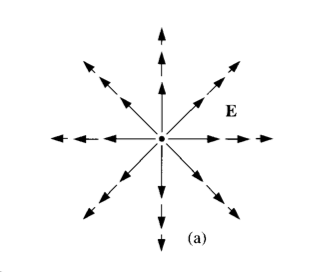
\includegraphics[width=0.99\textwidth]{./images/schematics/electric_field_pos_point_charge.png}\\
   \end{center}
  \end{column}
  \begin{column}{0.80\textwidth}
     As we know, the potential field $V(\vec{r})$ due to an
     {\bf electric monopole} (i.e. a point charge q) has an $1/r$ dependence:
     \begin{equation*}
         V = \frac{1}{4\pi\epsilon_0} \frac{q}{r}
     \end{equation*}
     Consequently, its electric field $\vec{E}(\vec{r})$ ($\vec{E} = -\vec{\nabla}V$)
     has an $1/r^2$ dependence.
  \end{column}
\end{columns}

\vspace{0.3cm}

\begin{columns}
  \begin{column}{0.80\textwidth}
     We will see that the potential field $V(\vec{r})$ due to an {\bf electric dipole} is
     \begin{equation*}
        {\bf V \approx \frac{1}{4\pi\epsilon_0} \frac{\vec{p} \hat{r}}{r^2} }
     \end{equation*}
     Therefore, it falls off as $1/r^2$, faster than the monopole potential.
     Consequently, the dipole electric field $\vec{E}(\vec{r})$
     has an $1/r^3$ dependence.
  \end{column}
  \begin{column}{0.20\textwidth}
   \begin{center}
     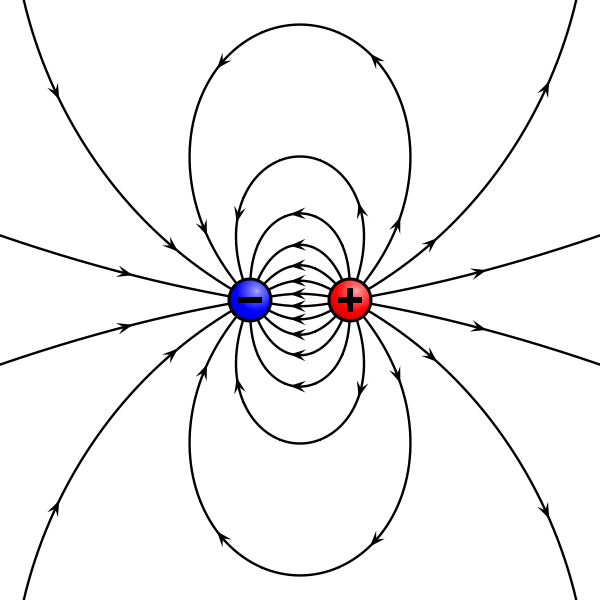
\includegraphics[width=0.90\textwidth]{./images/schematics/electric_dipole_field_lines_2.png}\\
   \end{center}
  \end{column}
\end{columns}

\end{frame}


%
%
%

\begin{frame}{Calculating the electric dipole field}

As we know, the potential field due to a single charge q is given by:
\begin{equation*}
  V = \frac{1}{4\pi\epsilon_0} \frac{q}{r}
\end{equation*}

\vspace{0.1cm}

\begin{columns}
  \begin{column}{0.25\textwidth}
   \begin{center}
     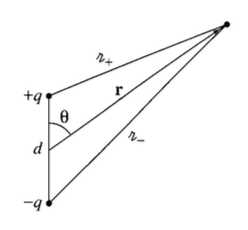
\includegraphics[width=0.95\textwidth]{./images/schematics/electric_dipole_0.png}\\
   \end{center}
  \end{column}
  \begin{column}{0.75\textwidth}
    Now, I have 2 charges: a positive and a negative one. The superposition principle applies.
    The potential at a distance r from the centre of the dipole is:
    \begin{equation*}
      V = \frac{1}{4\pi\epsilon_0} \Big( \frac{q}{r_{+}} - \frac{q}{r_{-}} \Big)
    \end{equation*}
  \end{column}
\end{columns}

\vspace{0.1cm}

I need to express $r_{+}$ and $r_{-}$ in terms of r.
From the law of cosines (generalisation of the Pythagorean theorem):
\begin{equation*}
  r_{+}^{2} = r^{2} + (d/2)^{2} - r \cdot d \cdot cos\theta
            = r^{2} \Big( 1 - \frac{d}{r} cos\theta + \frac{d^2}{4r^2} \Big) \xRightarrow{r>>d}
\end{equation*}
\begin{equation*}
   r_{+}^{2} \approx r^{2} \Big( 1 - \frac{d}{r} cos\theta \Big)
\end{equation*}

\end{frame}

%
%
%

\begin{frame}{Calculating the electric dipole field}

For $r_{-}$, the expressions are similar but involves $cos(\pi - \theta) = -cos\theta$ and,
therefore, there is an extra minus sign.
\begin{equation*}
   r_{-}^{2} \approx r^{2} \Big( 1 + \frac{d}{r} cos\theta \Big)
\end{equation*}

For convenience let me rename the small term involving d/r as $\epsilon$:
\begin{equation*}
  \frac{d}{r} cos\theta = \epsilon
\end{equation*}

We have that
\begin{equation*}
   r_{+}^{2} \approx r^{2} (1 - \epsilon) \Rightarrow
   r_{+} \approx r (1 - \epsilon)^{1/2} \Rightarrow
   \frac{1}{r_{+}} \approx \frac{1}{r} (1 - \epsilon)^{-1/2} \Rightarrow
   \frac{1}{r_{+}} \approx \frac{1}{r} (1 + \frac{1}{2}\epsilon)
\end{equation*}

and, similarly
\begin{equation*}
   \frac{1}{r_{-}} \approx \frac{1}{r} (1 - \frac{1}{2}\epsilon)
\end{equation*}

\end{frame}

%
%
%

\begin{frame}{Calculating the electric dipole field}

Therefore
\begin{equation*}
  \frac{1}{r_{+}} - \frac{1}{r_{-}} \approx
    \Big( \frac{1}{r} (1 + \frac{1}{2}\epsilon) \Big) -
    \Big( \frac{1}{r} (1 - \frac{1}{2}\epsilon) \Big) =
    \frac{1}{r} \epsilon \xRightarrow{\epsilon = \frac{d}{r} cos\theta}
\end{equation*}
\begin{equation*}
  \frac{1}{r_{+}} - \frac{1}{r_{-}} \approx \frac{d}{r^2} cos\theta
\end{equation*}

The electric dipole potential is given by
\begin{equation*}
  V = \frac{1}{4\pi\epsilon_0} \Big( \frac{q}{r_{+}} - \frac{q}{r_{-}} \Big) \Rightarrow
  V \approx \frac{1}{4\pi\epsilon_0} \frac{q d cos\theta}{r^2} \Rightarrow
\end{equation*}
\begin{equation*}
  V \approx \frac{1}{4\pi\epsilon_0} \frac{\vec{p} \cdot \hat{r}}{r^2}
\end{equation*}

So the potential of a dipole falls off as $1/r^2$ ($1/r$ for a monopole).\\
Consequently, the electric field of a dipole falls off as $1/r^3$.\\

\end{frame}

% ------------------------------------------------------------------------------

%
%
%

\begin{frame}{The {\em multipole} expansion}

\begin{columns}
  \begin{column}{0.30\textwidth}
   \begin{center}
     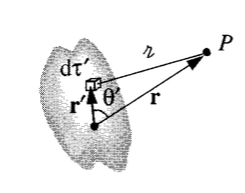
\includegraphics[width=0.99\textwidth]{./images/schematics/continuous_charge_distribution_1.png}\\
   \end{center}
  \end{column}
  \begin{column}{0.70\textwidth}
    For an {\bf arbitrary charge distribution} characterised by a density $\rho$
    the potential can be expanded to:
    \begin{equation*}
      V(r) = \frac{1}{4\pi\epsilon_0} \sum_{n=0}^{\infty} \frac{1}{r^{n+1}}
        \int_{vol} (r^{\prime})^{n} P_{n}(cos\theta^{\prime}) \rho(\vec{r^{\prime}}) d{\tau}^{\prime}
    \end{equation*}
    where $\theta^{\prime}$ is the angle between $\vec{r}$ and $\vec{r^{\prime}}$.
    Notice that there is no r dependence in the integral.\\
  \end{column}
\end{columns}

\vspace{0.3cm}

This is called the {\bf multipole expansion}.
\begin{itemize}
{\small
  \item The first ($1/r$) term is the {\bf monopole} term
  \item The second ($1/r^2$) term is the {\bf dipole} term
  \item $1/r^3$ term: {\bf quadruple} term
  \item $1/r^4$ term: {\bf octopole} term
  \item ...
}
\end{itemize}

\end{frame}

% ------------------------------------------------------------------------------

%
% Worked example : The not-so-parallel plate capacitor
%

{
\problemslide

\begin{frame}{Worked example: The not-so-parallel plate capacitor}

  \begin{blockexmplque}{Question}
  In the figure below, you are given the not-so-parallel plate capacitor.
  \begin{itemize}
    \item
     Neglecting edge effects, when a voltage difference $V_0$ is placed
     across the two conductors, find the potetial everywhere between the plates.
    \item
     When the wedge is filled with a medium of dielectric constant $\epsilon$,
     find the capacitance of the system in terms of the constants given.
  \end{itemize}
  \begin{center}
    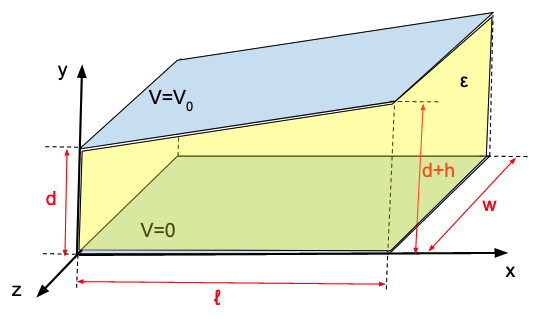
\includegraphics[width=0.60\textwidth]{./images/problems/lect4_not_so_parallel_plane_capacitor_1.png}\\
  \end{center}
  \end{blockexmplque}

\end{frame}

%
%
%

\begin{frame}{Worked example: The not-so-parallel plate capacitor}

Neglecting edge effects, the problem is a two-dimensional one.\\
\vspace{0.1cm}
Symmetry dictates that the electric field is parallel to the $xy$ plane
and it is {\em independent} of $z$.\\
\vspace{0.1cm}
A convenient coordinate system for our analysis is $O^\prime (x^\prime, y^\prime, z^\prime)$
which is shifted from $O (x, y, z)$ by a distance $\ell^\prime$ along the $x$ axis,
so imaginary extrapolations of the capacitor plates
intersect at $x^\prime=0$, as shown below.

\begin{center}
  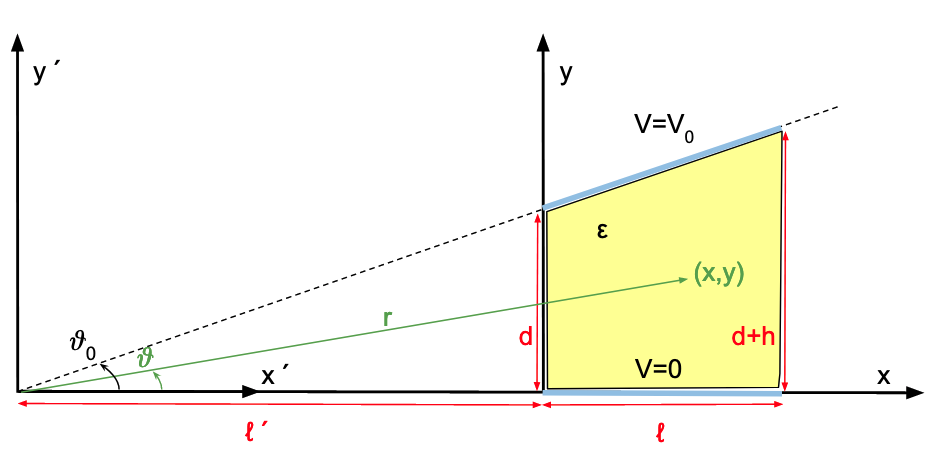
\includegraphics[width=0.80\textwidth]{./images/problems/lect4_not_so_parallel_plane_capacitor_2.png}\\
\end{center}

\end{frame}


%
%
%

\begin{frame}{Worked example: The not-so-parallel plate capacitor}

The quantities $\ell^\prime$, $\theta_0$, $\theta$ and $r$ introduced above (see schematic)
can be easily related to the given quantities $\ell$, $d$, $h$ and the coordinates $x,y$
of a point within the capacitor in the original coordinate system ($O$).

  \begin{equation*}
    tan\theta_0 = \frac{d+h}{\ell+\ell^\prime} = \frac{d}{\ell^\prime} \Rightarrow
     \ell^\prime = \ell \frac{d}{h}
  \end{equation*}

  \begin{equation*}
    tan\theta_0 = \frac{d}{\ell^\prime} = \frac{\cancel{d}}{\ell \frac{\cancel{d}}{h}} \Rightarrow
    \theta_0 = arctan\Big(\frac{h}{\ell}\Big)
  \end{equation*}

  \begin{equation*}
    tan\theta = \frac{y}{x+\ell^\prime} = \frac{y}{x+\ell \frac{d}{h}} \Rightarrow
    \theta = arctan\Big(\frac{y}{x+\ell \frac{d}{h}}\Big)
  \end{equation*}

  \begin{equation*}
    cos\theta = \frac{x+\ell^\prime}{r} = \frac{x+\ell \frac{d}{h}}{r} \xRightarrow{\; cos\theta \approx 1 \;}
    r = x + \ell \frac{d}{h}
  \end{equation*}

\end{frame}

%
%
%

\begin{frame}{Worked example: The not-so-parallel plate capacitor}

The potetial between the plates can be found by solving Poisson's equation

  \begin{equation*}
    \vec{\nabla}^{2} V = \frac{\rho}{\epsilon_0} \xRightarrow{\rho=0}
    \vec{\nabla}^{2} V = 0
  \end{equation*}

In polar coordinates, this is written as

  \begin{equation*}
    \frac{1}{r^2} \frac{d^2V(\theta)}{d\theta} = 0 \Rightarrow
    \frac{d^2V(\theta)}{d\theta} = 0
  \end{equation*}

\vspace{0.2cm}

The equation has the following solution

  \begin{equation*}
    V(\theta) = A + B \theta
  \end{equation*}

The costants $A, B$ can be derived from the boundary conditions

  \begin{equation*}
    V(\theta = 0) = 0 \Rightarrow A = 0
  \end{equation*}

  \begin{equation*}
    V(\theta = \theta_0) = V_0 \xRightarrow{A = 0}
    B \theta_0 = V_0 \Rightarrow B = \frac{V_0}{\theta_0}
  \end{equation*}

\end{frame}

%
%
%

\begin{frame}{Worked example: The not-so-parallel plate capacitor}

Therefore, the solution $V(\theta)$ is given by

  \begin{equation*}
    V(\theta) =  \frac{V_0}{\theta_0} \theta
  \end{equation*}

Using the expression for $\theta_0$ that was derived previously,
$V(\theta)$ can be written as

  \begin{equation*}
    V(\theta) =  \frac{V_0}{arctan\Big(\frac{h}{\ell}\Big)} \theta
  \end{equation*}

In terms of coordinates $x,y$ in the original coordinate system ($O$),
the potential can be expressed as

  \begin{equation*}
    V(x,y) =  \frac{V_0}{arctan\Big(\frac{h}{\ell}\Big)}
     \arctan\Big(\frac{y}{x+\ell \frac{d}{h}}\Big)
  \end{equation*}

\end{frame}

%
%
%

\begin{frame}{Worked example: The not-so-parallel plate capacitor}

The capacitance of the system will be calculated from
  \begin{equation*}
    C = \frac{|Q|}{|V_0|}
  \end{equation*}

where the unknown charge $Q$ can be estimated from
  \begin{equation*}
    Q = \oint \vec{D} \cdot d\vec{S}
  \end{equation*}

The field $\vec{D}$ is related to electric field $\vec{E}$,
and therefore the potential V, as
  \begin{equation*}
    \vec{D} = \epsilon \vec{E} \xRightarrow{\vec{E} = -\vec{\nabla}V}
    \vec{D} = -\epsilon \vec{\nabla}V
  \end{equation*}

Therefore
  \begin{equation*}
    \vec{D} =
      -\epsilon \frac{1}{r} \frac{\partial V}{\partial \theta} \hat{\theta}
      \xRightarrow{\;V =  \frac{V_0}{\theta_0} \theta \;}
    \vec{D} = - \frac{1}{r} \frac{\epsilon V_0}{\theta_0} \hat{\theta}
  \end{equation*}

\end{frame}

%
%
%

\begin{frame}{Worked example: The not-so-parallel plate capacitor}

Using the above expression for $\vec{D}$, $Q$ is calculated as
  \begin{equation*}
    Q = \oint \vec{D} \cdot d\vec{S} = \oint D dS
     \xRightarrow{\; dS = w dx, \; D = - \frac{1}{r} \frac{\epsilon V_0}{\theta_0} \;}
     Q = -\frac{w \epsilon V_0}{\theta_0} \int_{0}^{\ell} \frac{1}{r} dx
      \xRightarrow{\; r = x + \ell \frac{d}{h} \;}
  \end{equation*}

  \begin{equation*}
    Q = -\frac{w \epsilon V_0}{\theta_0} \int_{0}^{\ell} \frac{1}{x + \ell \frac{d}{h}} dx =
        -\frac{w \epsilon V_0}{\theta_0} ln(x + \ell \frac{d}{h}) \Big\rvert_{0}^{\ell} \Rightarrow
  \end{equation*}

  \begin{equation*}
    Q = -\frac{w \epsilon V_0}{\theta_0} ln \frac{d + h}{d}
    \xRightarrow{\theta_0 = arctan\Big(\frac{h}{\ell}\Big)}
    Q = -\frac{w \epsilon V_0}{arctan\Big(\frac{h}{\ell}\Big)} ln \Big(\frac{d + h}{d}\Big)
  \end{equation*}

Therefore
  \begin{equation*}
    C = \frac{|Q|}{|V_0|} =
      \frac{w \epsilon}{arctan\Big(\frac{h}{\ell}\Big)} ln \Big(\frac{d + h}{d}\Big)
  \end{equation*}

\end{frame}


} % Worked example

% ------------------------------------------------------------------------------

%
% Worked example : Pulling a dielectric out of a capacitor
%

{
\problemslide

\begin{frame}{Worked example: Pulling a dielectric out of a capacitor}

  \begin{blockexmplque}{Question}
  A cylindrical capacitor of length $L$ consists of an inner metallic wire
  of radius $a$, and a thin outer metallic shell of radius $b$.
  The space in between is filled with a dielectric with permittivity $\epsilon$.\\
  As we have seen in the workshops, if edge effects are ignored,
  the capacitance $C$ of the cylindrical
  capacitor is given by
  \begin{equation*}
    C = \frac{2\pi \epsilon L}{ln(b/a)}.
  \end{equation*}
  \vspace{0.2cm}
  Suppose that the dielectric is pulled partly out of the capacitor,
  and that the capacitor is connected to a battery of electromotive force $V$.
  \begin{enumerate}
  \item
  Find the force necessary to hold the dielectric in this position.
  \item
  In which direction must the force be applied?\\
  \end{enumerate}
  \end{blockexmplque}

\end{frame}

%
%
%

\begin{frame}{Worked example: Pulling a dielectric out of a capacitor}

  \begin{center}
    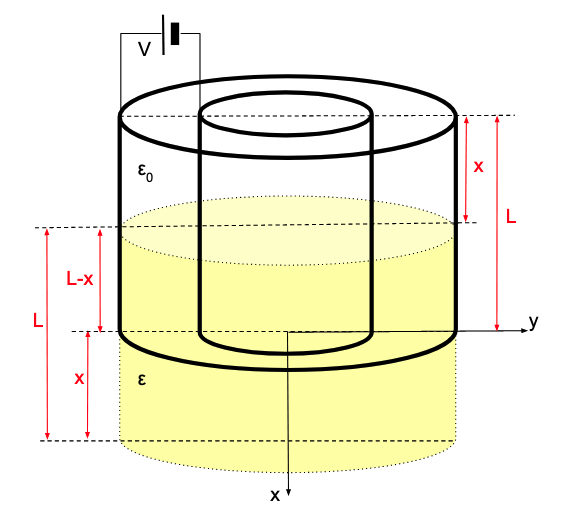
\includegraphics[width=0.67\textwidth]{./images/problems/lect4_pulling_dielectric_out_of_capacitor_1.png}\\
  \end{center}

\end{frame}

%
%
%

\begin{frame}{Worked example: Pulling a dielectric out of a capacitor}

  If the dielectric is pulled out of the cylindrical capacitor by a length $x$,
  then length $L-x$ remains inside the capacitor.

  The part of the capacitor with length $x$ that does not have a dielectric
  has capacitance $C_1$ given by
  \begin{equation*}
    C_1 = \frac{2\pi \epsilon_0 x}{ln(b/a)}
  \end{equation*}
  whereas the part of the capacitor with length $L-x$ that does have a
  dielectric has a capacitance $C_2$ given by
  \begin{equation*}
    C_2 = \frac{2\pi \epsilon (L-x)}{ln(b/a)}.
  \end{equation*}

  Those two capacitors have a common potential difference across the
  inner and outer conductors (connected parallel) and, therefore, the
  combined capacitance $C$ is
  \begin{equation*}
    C = C_1 + C2 =
     \frac{2\pi \epsilon_0 x}{ln(b/a)} +
     \frac{2\pi \epsilon (L-x)}{ln(b/a)} =
     \frac{2\pi \epsilon}{ln(b/a)}
         \Big(L + (\frac{\epsilon_0}{\epsilon}-1) x \Big)
  \end{equation*}

\end{frame}

%
%
%

\begin{frame}{Worked example: Pulling a dielectric out of a capacitor}

  The work provided by the battery as it charges the capacitor
  becomes energy stored in the capacitor and mechanical work of
  the force $F$ that moves the dielectric with respect to the capacitor.
  We can write
  \begin{equation*}
    dW_{battery} = dU_{capacitor} + dW_{mechanical} \Rightarrow
  \end{equation*}
  \begin{equation*}
    V dQ = d\Big(\frac{1}{2}CV^2\Big) + F dx
  \end{equation*}
  Since $V$ is constant, the above can be written as
  \begin{equation*}
    V dQ = \frac{1}{2}V^2 dC + F dx
  \end{equation*}
  Using the definition of capacitance, $C = \frac{Q}{V}$, we can write
  \begin{equation*}
    dC = \frac{dQ}{V} \Rightarrow V^2 dC = V dQ
  \end{equation*}
  From all the above, we obtain
  \begin{equation*}
    V^2 dC = \frac{1}{2}V^2 dC + F dx \Rightarrow
    \frac{1}{2}V^2 dC = F dx
  \end{equation*}

\end{frame}

%
%
%

\begin{frame}{Worked example: Pulling a dielectric out of a capacitor}

  As the dielectric exits the capacitor, $x$ increases
  and, therefore, $dx > 0$.

  When $x$ increases we expect the capacitance $C$ to decrease.
  Given that $\epsilon_0/\epsilon < 1$,
  this can be easily deduced from the expression for $C$,
  \begin{equation*}
    C =
     \frac{2\pi \epsilon}{ln(b/a)}
         \Big(L + (\frac{\epsilon_0}{\epsilon}-1) x \Big).
  \end{equation*}
  Therefore, for $dx > 0$, $dC < 0$.
  Considering this and observing the expression
  \begin{equation*}
    \frac{1}{2}V^2 dC = F dx,
  \end{equation*}
  we see that the term $F dx$ needs to be negative.
  Therefore, for $dx > 0$ (direction of exiting the capacitor),
  the direction of the force on the dielectric is opposite,
  and the dielectric is pulled into the capacitor.

  If we wanted to hold the dielectric in a fixed position, we would
  need to apply an opposite force $\vec{F^\prime}(=-\vec{F})$,
  pointing {\em away} from the capacitor.

\end{frame}

%
%
%

\begin{frame}{Worked example: Pulling a dielectric out of a capacitor}

  The magnitude of my force $F^\prime=F$
  \begin{equation*}
    \frac{1}{2}V^2 dC = F dx \Rightarrow
    F = \frac{1}{2}V^2 \frac{dC}{dx}
  \end{equation*}

  Differentiating the expression for $C$ we derived earlier, we find
  \begin{equation*}
    \frac{dC}{dx} = \frac{2\pi \epsilon}{ln(b/a)}
        \Big(\frac{\epsilon_0}{\epsilon}-1\Big)
  \end{equation*}

  Thefore, the magnitude of the force is given by
  \begin{equation*}
    F = \frac{1}{2}V^2 \frac{2\pi \epsilon}{ln(b/a)}
     \Big(\frac{\epsilon_0}{\epsilon}-1\Big) \Rightarrow
    F = \frac{\pi \epsilon V^2}{ln(b/a)}
      \Big(\frac{\epsilon_0}{\epsilon}-1\Big)
  \end{equation*}

\end{frame}

} % Worked example

% ------------------------------------------------------------------------------

%
% Worked example : Spherical capacitor with inhomogeneous dielectric
%

{
\problemslide

\begin{frame}{Worked example: Cylindrical and spherical capacitors}

  \begin{blockexmplque}{Question}
  Calculate the capacitance of a cylindrical and a spherical capacitor.\\
  \begin{columns}
    \begin{column}{0.60\textwidth}
     \begin{center}
       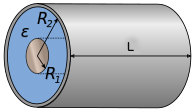
\includegraphics[width=0.75\textwidth]{./images/schematics/capacitors_cylindrical_1.png}\\
       \begin{equation*}
           C = \frac{2 \pi \epsilon L}{ln(R_2/R_1)}
       \end{equation*}
     \end{center}
    \end{column}
    \begin{column}{0.40\textwidth}
     \begin{center}
       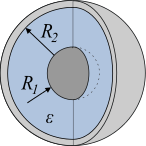
\includegraphics[width=0.75\textwidth]{./images/schematics/capacitors_spherical_1.png}\\
       \begin{equation*}
           C = \frac{4 \pi \epsilon}{\frac{1}{R_1}-\frac{1}{R_2}}
       \end{equation*}
     \end{center}
    \end{column}
  \end{columns}
  \end{blockexmplque}

\end{frame}

%
%
%

\begin{frame}{Worked example: Cylindrical and spherical capacitors}

  %-----------
  % cylindrical
  %-----------

  As a Gaussian surface, for the calculation for a cylindrical capacitor,
  we choose a cylinder of length $L$
  and radius $\rho$ ($R_1$ $\le$ $\rho$ $\le$ $R_2$), closed by end caps.
  It is coaxial with the cylinders of radii $R_1$ and $R_2$ and
  encloses the central cylinder and
  thus also the charge $Q$ on that cylinder.
  Let's assume, without loss of generality, that the inner conductor is
  positively charged and the outer conductor is negatively charged.

  From Gauss' law:
  \begin{equation*}
    \Phi_E = Q/\epsilon_0 \Rightarrow
    \oint_{S} \vec{E} \cdot d\vec{S} = Q/\epsilon_0
  \end{equation*}

  The electric field $\vec{E}$
  is collinear with the normal to the Gaussian surface and, due to
  cylindrical symmetry, it has the same magnitude everywhere on that
  surface. There is no electric flux through the end caps.\\
  The overall flux through the closed Gaussian surface is:
  \begin{equation*}
    \oint_{S} \vec{E} \cdot d\vec{S} =
    \oint_{S} E \cdot dS =
    E \oint_{S} dS =
    E S = E (2\pi \rho L)
  \end{equation*}

\end{frame}

%
%
%

\begin{frame}{Worked example: Cylindrical and spherical capacitors}

  Therefore:
  \begin{equation*}
    E (2\pi \rho L) = Q/\epsilon_0 \Rightarrow
    E = \frac{Q}{2\pi \epsilon_0 L \rho}
  \end{equation*}

  In vector form the electric field is written as:
  \begin{equation*}
    \vec{E} = \frac{Q}{2\pi \epsilon_0 L \rho} \cdot \hat{\rho}
  \end{equation*}
  where $\hat{\rho}$ is the axial radial unit vector of the cylindrical
  coordinate system used (it is perpendicular to the axis of the
  two cylindrical conductors and it points outwards).\\

  The potential difference $V$ between the positively and negatively
  charged conductors is:
  \begin{equation*}
      V := V_{+} - V_{-} = - \int_{-}^{+} \vec{E} \cdot d\vec{\ell}
  \end{equation*}

  This integral is path-independent.
  The integral is simplified if $\vec{E}$ and $d\vec{\ell}$ are colinear.
  Since the electric field points along  $\hat{\rho}$, we chose
  $d\vec{\ell} = d\rho \cdot \hat{\rho}$.\\

\end{frame}

%
%
%

\begin{frame}{Worked example: Cylindrical and spherical capacitors}

  Therefore:
  \begin{equation*}
      V = - \frac{Q}{2\pi \epsilon_0 L} \int_{R_2}^{R_1} \frac{d\rho}{\rho}
  \end{equation*}

  \begin{equation*}
        = -  \frac{Q}{2\pi \epsilon_0 L} ln(\rho) \rvert_{R_2}^{R_1} =
          - \frac{Q}{2\pi \epsilon_0 L}  (ln R_1 - ln R_2) =
            \frac{Q}{2\pi \epsilon_0 L}  (ln R_2 - ln R_1) \Rightarrow
  \end{equation*}

  \begin{equation*}
        V = \frac{Q}{2\pi \epsilon_0 L}  ln(R_2/R_1)
  \end{equation*}

  Therefore, the capacitance of a cylindrical capacitor is given by:
  \begin{equation*}
      C = \frac{Q}{V} = \frac{Q}{\frac{Q}{2\pi \epsilon_0 L}  ln(R_2/R_1)} =
             2\pi \epsilon_0 \frac{L}{ln(R_2/R_1)}
  \end{equation*}

\end{frame}

%
%
%

\begin{frame}{Worked example: Cylindrical and spherical capacitors}

  %-----------
  % spherical
  %-----------

  As a Gaussian surface, for the calculation for a spherical capacitor,
  we choose a sphere of radius $r$ ($R_1$ $\le$ $r$ $\le$ $R_2$)
  which is concentric with the spherical shells of radii $R_1$ and $R_2$.
  Let's assume, without loss of generality, that the inner conductor is
  positively charged and the outer conductor is negatively charged.

  From Gauss' law:
  \begin{equation*}
    \Phi_E = Q/\epsilon_0 \Rightarrow
    \oint_{S} \vec{E} \cdot d\vec{S} = Q/\epsilon_0
  \end{equation*}

  The electric field $\vec{E}$
  is collinear with the normal to the chosen Gaussian surface and, due to
  spherical symmetry, it has the same magnitude everywhere on that
  surface:
  \begin{equation*}
    \oint_{S} \vec{E} \cdot d\vec{S} =
    \oint_{S} E \cdot dS =
    E \oint_{S} dS =
    E S =
    E (4\pi r^2)
  \end{equation*}

\end{frame}

%
%
%

\begin{frame}{Worked example: Cylindrical and spherical capacitors}

  Therefore:
  \begin{equation*}
    E (4\pi r^2) = Q/\epsilon_0 \Rightarrow
    E = \frac{Q}{4\pi \epsilon_0 r^2}
  \end{equation*}

  In vector form the electric field is written as:
  \begin{equation*}
    E = \frac{Q}{4\pi \epsilon_0 r^2} \hat{r}
  \end{equation*}
  where $\hat{r}$ is the radial unit vector of the spherical coordinate
  system used.

  The potential difference $V$ between the positively and negatively
  charged conductors is:
  \begin{equation*}
      V := V_{+} - V_{-} = - \int_{-}^{+} \vec{E} d\vec{\ell}
  \end{equation*}

  The above path-independent integral is
  simplified if $\vec{E}$ and $d\vec{\ell}$ are collinear
  ($d\vec{\ell} = dr \cdot \hat{r}$).

\end{frame}

%
%
%

\begin{frame}{Worked example: Cylindrical and spherical capacitors}

  Therefore:
  \begin{equation*}
      V = - \frac{Q}{4\pi} \int_{R_2}^{R_1}  \frac{dr}{r^2}
  \end{equation*}

  \begin{equation*}
        =   - \frac{Q}{4\pi \epsilon_0}  (-\frac{1}{r}) \rvert_{R_2}^{R_1} =
            - \frac{Q}{4\pi \epsilon_0}  (-\frac{1}{R_1} + \frac{1}{R_2}) =
            \frac{Q}{4\pi \epsilon_0}   (\frac{1}{R_1} - \frac{1}{R_2}) \Rightarrow
            \frac{Q}{4\pi \epsilon_0} \frac{R_2-R_1}{R_1 R_2}
  \end{equation*}

  \begin{equation*}
        V = \frac{Q}{4\pi \epsilon_0} \frac{R_2-R_1}{R_1 R_2}
  \end{equation*}

  Therefore, the capacitance of a spherical capacitor is given by:
  \begin{equation*}
      C = \frac{Q}{V} = \frac{Q}{\frac{Q}{4\pi \epsilon_0} \frac{R_2-R_1}{R_1 R_2}} =
             4\pi \epsilon_0 \frac{R_1 R_2}{R_2-R_1}
  \end{equation*}

\end{frame}

} % Worked example

% ------------------------------------------------------------------------------

%
% Worked example : Spherical capacitor with inhomogeneous dielectric
%

{
\problemslide

%
%
%

\begin{frame}{Worked example: Capacitor with inhomogeneous dielectric}

  \begin{blockexmplque}{Question}
    The volume between two concentric conducting spherical surfaces of
    radii $a$ and $b$ $(a < b)$, is filled with an inhomogeneous dielectric
    with permittivity
    \begin{equation*}
       \epsilon = \frac{\epsilon_0}{1+Kr}
    \end{equation*}
    where $K$ is a constant and $r$ is the radial coordinate.
    The displacement field $\vec{D}$ is related to the electric
    field $\vec{E}$ by the usual formula $\vec{D} = \epsilon \vec{E}$.\\
    A charge $Q$ is placed on the inner surface,
    while the outer one is grounded.\\
    Find:
    \begin{itemize}
      \item The magnitude and direction of the electric displacement
       in the region $a < r < b$.
      \item The capacitance of the device.
      \item The volume polarization charge density in $a < r < b$.
      \item The surface polarization charge density at $r = a$ and $r = b$.
    \end{itemize}
  \end{blockexmplque}

\end{frame}

%
%
%

\begin{frame}{Worked example: Capacitor with inhomogeneous dielectric}

  The integral form of Gauss's law for the electric displacement field
  $\vec{D}$ is
  \begin{equation*}
    \oint \vec{D} \cdot d\vec{S} = Q_{free}
  \end{equation*}

  Due to spherical symmetry of the problem, if we choose as integration
  surface the surface of a sphere of radius r (a < r < b),
  the vectors $\vec{D}$ and $d\vec{S}$ are both radial,
  and $|\vec{D}|=D$ is constant over the integration surface.
  Therefore:
  \begin{equation*}
    \oint D dS = Q_{free}  \Rightarrow
     D \oint dS = Q_{free} \Rightarrow
     D 4 \pi r^2 = Q_{free} \Rightarrow
  \end{equation*}

  \begin{equation*}
     D(r) = \frac{Q_{free}}{4\pi r^2}
  \end{equation*}

  The radial vector $\vec{D}$ can be written in vector form as:
  \begin{equation*}
     \vec{D}(\vec{r}) = \frac{Q_{free}}{4\pi r^2} \hat{r}
  \end{equation*}

\end{frame}

%
%
%

\begin{frame}{Worked example: Capacitor with inhomogeneous dielectric}

  The displacement and electric field vectors are related by:
  \begin{equation*}
     \vec{D}(\vec{r}) = \epsilon \vec{E}(\vec{r})
  \end{equation*}

  Therefore:
  \begin{equation*}
     \vec{E}(\vec{r}) = \frac{Q_{free}}{4\pi \epsilon r^2} \hat{r}
%     \label{eq:p2b_Evec1}
  \end{equation*}

  The expression given for the permittivity of the inhomogeneous
  dielectric is
  \begin{equation*}
     \epsilon = \frac{\epsilon_0}{1+Kr}
%     \label{eq:p2_epsilon}
  \end{equation*}

  Substituting the above expression for $\epsilon$
  into the earlier expression for $\vec{E}$, we have:
  \begin{equation*}
     \vec{E}(\vec{r}) = \frac{Q_{free}}{4\pi \epsilon_0} \frac{1+Kr}{r^2} \hat{r}
%     \label{eq:p2b_Evec2}
  \end{equation*}

\end{frame}

%
%
%

\begin{frame}{Worked example: Capacitor with inhomogeneous dielectric}

  The potential difference $V$ between the two concentric spherical
  surfaces of radii a and b is given by:
  \begin{equation*}
     V = \int_{a}^{b} \vec{E}(\vec{r}) \cdot d\vec{\ell}
%     \label{eq:p2b_V1}
  \end{equation*}

  Choosing a radial integration path:
  \begin{equation*}
    d\vec{\ell}=d\vec{r}
  \end{equation*}

  and carrying out the integration from a to b, we find:
  \begin{equation*}
     V =
     \frac{Q_{free}}{4\pi \epsilon_0} \int_{a}^{b} \frac{1+Kr}{r^2} \hat{r} \cdot d\vec{r} =
     \frac{Q_{free}}{4\pi \epsilon_0} \int_{a}^{b} \frac{1+Kr}{r^2} dr =
     \frac{Q_{free}}{4\pi \epsilon_0}
       \Big( \int_{a}^{b} \frac{dr}{r^2} + K \int_{a}^{b} \frac{dr}{r} \Big)
  \end{equation*}

  \begin{equation*}
       = \frac{Q_{free}}{4\pi \epsilon_0}
       \Big( -\frac{1}{r} + K ln(r) \Big) \Bigg\rvert_{a}^{b} =
         \frac{Q_{free}}{4\pi \epsilon_0}
       \Big( -\frac{1}{b} + K ln(b) + \frac{1}{a} - K ln(a) \Big) \Rightarrow
  \end{equation*}

\end{frame}

%
%
%

\begin{frame}{Worked example: Capacitor with inhomogeneous dielectric}

  \begin{equation*}
     V = \frac{Q_{free}}{4\pi \epsilon_0}
       \Big( \frac{1}{a} - \frac{1}{b} + K ln(\frac{b}{a}) \Big)
%       \label{eq:p2b_V2}
  \end{equation*}

  The capacitance of the device is given by:
  \begin{equation*}
     C = \frac{Q_{free}}{V}
  \end{equation*}

  Substituting V, we find:
  \begin{equation*}
     \displaystyle
     C = \frac{\cancel{Q_{free}}}{
       \frac{\cancel{Q_{free}}}{4\pi \epsilon_0}
          \Big( \frac{1}{a} - \frac{1}{b} + K ln(\frac{b}{a}) \Big) }
       = \frac{4\pi\epsilon_0}
              {\frac{1}{a} - \frac{1}{b} + K ln(\frac{b}{a})} \Rightarrow
  \end{equation*}

  \begin{equation*}
     \displaystyle
     C = \frac{4\pi\epsilon_0 a b}{b - a + K a b ln(\frac{b}{a})}
  \end{equation*}

\end{frame}
%
%
%

\begin{frame}{Worked example: Capacitor with inhomogeneous dielectric}

  The polarization vector $\vec{P}$ is given by:
  \begin{equation*}
     \vec{P} = \chi_{e} \epsilon_0 \vec{E}
%     \label{eq:p2c_P1}
  \end{equation*}

  The factor $\chi_{e} \epsilon_0$ can be expressed in terms of
  the given $\epsilon$ as follows:
  \begin{equation*}
     1+\chi_{e} = \epsilon_{r} = \frac{\epsilon}{\epsilon_0} \Rightarrow
     (1+\chi_{e})\epsilon_0 = \epsilon \Rightarrow
     \chi_{e} \epsilon_0 = \epsilon - \epsilon_0
  \end{equation*}

  Using the above, the earlier expression for $\vec{P}$ can be written as:
  \begin{equation*}
     \vec{P} = (\epsilon - \epsilon_0) \vec{E}
%     \label{eq:p2c_P2}
  \end{equation*}

  Substituting the given expression of $\epsilon$, we have:
  \begin{equation*}
     \vec{P} =
        (\frac{\cancel{\epsilon_0}}{1+Kr} - \cancel{\epsilon_0})
        \frac{Q_{free}}{4\pi\cancel{\epsilon_0}} \frac{1+Kr}{r^2} \hat{r} =
        \frac{Q_{free}}{4\pi}
        \Big(\frac{1}{1+Kr} - 1\Big)
        \frac{1+Kr}{r^2} \hat{r}
  \end{equation*}

  \begin{equation*}
    = \frac{Q_{free}}{4\pi}
      \frac{\cancel{1}-\cancel{1}-K\cancel{r}}{\cancel{1+Kr}}
      \frac{\cancel{1+Kr}}{r^{\cancel{2}}} \hat{r} \Rightarrow
     \vec{P} = - \frac{Q_{free}K}{4\pi r} \hat{r}
  \end{equation*}

\end{frame}
%
%
%

\begin{frame}{Worked example: Capacitor with inhomogeneous dielectric}

  The volume polarization charge density $\rho_{P}$ is given by:

  \begin{equation*}
     \rho_{P} = - \vec{\nabla} \cdot \vec{P}
  \end{equation*}

  Substituting in the above equation the expression for $\vec{P}$, we have:
  \begin{equation*}
     \rho_{P} = - \vec{\nabla} \cdot \Big( - \frac{Q_{free}K}{4\pi r} \hat{r} \Big)
  \end{equation*}

  As $\vec{P}$ is radial vector, it is easier to evaluate its divergence
  expressing the divergence operator in spherical coordinates.
  Doing so, we find the volume polarization charge density $\rho_{P}$ to be
  \begin{equation*}
     \rho_{P} = - \frac{1}{r^2} \frac{\partial}{\partial r}
                  \Bigg(r^2
                    \Big( - \frac{Q_{free}K}{4\pi r} \Big)
                  \Bigg) \Rightarrow
  \end{equation*}

  \begin{equation*}
     \rho_{P} = \frac{Q_{free}K}{4\pi r^2}
  \end{equation*}

\end{frame}
%
%
%

\begin{frame}{Worked example: Capacitor with inhomogeneous dielectric}

  The surface polarization charge densities $\sigma_{P}$
  ar $r=a,b$ are given by the projection of $\vec{P}$
  along the corresponding surface vectors.

  Using the expression of $\vec{P}$ we found earlier, we get:

  \begin{equation*}
     \sigma_{P}(r=a) = \vec{P} \cdot (-\hat{r}) = \frac{Q_{free}K}{4\pi a}
  \end{equation*}

  and

  \begin{equation*}
     \sigma_{P}(r=b) = \vec{P} \cdot (+\hat{r}) = - \frac{Q_{free}K}{4\pi b}
  \end{equation*}

\end{frame}


} % Worked example

% ------------------------------------------------------------------------------
